\section{Постановка задачи и основные Результаты}
\label{sec:probl}

В этом разделе мы представляем наш алгоритм и фреймворк для построения CBM. Алгоритм, представленный в разделе \ref{sec:cms}, обеспечивает повышение точности CLIP наряду с его интерпретируемостью, а фреймворк (см. раздел \ref{sec:framework}) обеспечивает контрастную тонкую настройку магистрального бимодального кодера.

\subsection{Постановка задачи}

Наряду с задачей классификации изображений, мы формализуем классификацию с помощью \textbf{Concept Bottleneck}. Учитывая кодировщики изображений и текста, мы намерены выучить дополнительную проекцию из пространства вложений, предоставляемого кодировщиками, в векторное пространство, соответствующее представлению концептов изображений, а затем выучить окончательную проекцию для получения вероятностей меток классов. Мы намерены выучить следующее отображение: $x\times t \to \omega \to l$, согласно \textit{Notation} \ref{sec:notation}: $x$ обозначает область изображений, $t$ - текстовые понятия, а $\omega$ и $l$ - представление понятий и метки классов соответственно. Это отличается от стандартной схемы $x\to \omega\to l$ тем, что мы можем создавать концепты $t$ автоматизированным способом.

\subsection{Concept Matrix Search algorithm}\label{sec:cms}

Мы представляем алгоритм Concept Matrix Search (CMS), который использует возможности CLIP для представления изображений и текстов в совместном латентном пространстве одной и той же размерности. Сначала мы формулируем гипотезу о наших данных, принимая во внимание то, как обучена основная модель CLIP.

Определим набор эмбеддингов картинки как $\mathrm{I} = \{i_1, \dots, i_{|\mathrm{I}|}\}$, where $i_{\mathrm{k}} = f_{\mathrm{I}}(x_{\mathrm{k}}, \theta)$. И в качестве $\mathrm{D} = \{d_1, \dots, d_{|\mathrm{D}|}\}$ мы определим набор эмбеддингов концептов, $d_\mathrm{j} = f_{\mathrm{T}}(\mathrm{concept}_{\mathrm{j}}, \theta)$, тем временем $\mathrm{C} = \{c_1, \dots, c_{|\mathrm{C}|}\}$ набор эмбеддингов классов, где эмбеддинги меток этих классов похоже выражены iв терминах $f_{\mathrm{T}}$. Мы также определим две матрицы для которых наша модель будет вычислять попарную близость картинка-текст:

Image-Concept matrix (V-matrix): $\mathcal{V}\in \mathbb{R}^{|\mathrm{I}|\times|\mathrm{D}|}$, such that $\mathcal{V}_{\mathrm{kl}} =\langle i_\mathrm{k}, d_\mathrm{l}\rangle$.

Class-Concept matrix (T-matrix): $\mathcal{T}\in\mathbb{R}^{|\mathrm{C}|\times|\mathrm{D}|}$, such that $\mathcal{T}_{\mathrm{kl}} = \langle c_\mathrm{k}, d_\mathrm{l} \rangle$.

Теперь мы можем сформулировать \textit{гипотезу} лежащую в основынии CMS.

\paragraph{Гипотеза.}

Для $f_{\mathrm{I}}(x,\theta)$ and $f_{\mathrm{T}}(t,\theta)$ определим косинусную близость как:
\[ 
\cos(f_{\mathrm{I}}(x, \theta), f_{\mathrm{T}}(t, \theta)) = \frac{\langle f_{\mathrm{I}}(x, \theta), f_{\mathrm{T}}(t, \theta) \rangle}{\|f_{\mathrm{I}}(x, \theta)\| \|f_{\mathrm{T}}(t, \theta)\|}_.
\]

Тогда,
\begin{quote}
\textit{Для матриц} $\mathcal{V}$, $\mathcal{T}$ \textit{и функции} $\phi(\mathrm{m})\colon \mathbb{N}^{|\mathrm{I}|} \to \mathbb{N}^{|\mathrm{C}|}$ \textit{которая отображает индекс эмбеддинга картинки} $\mathcal{V}$ \textit{в индекс его класса из} $\mathcal{T}$\textit{, мы предполагаем:}
\[
\forall \mathrm{j}\neq \mathrm{k} \hookrightarrow \cos(\mathcal{V}_{\mathrm{k},\cdot}^\top, \mathcal{T}_{\phi(\mathrm{k}),\cdot}^\top) \geq \cos(\mathcal{V}_{\mathrm{k},\cdot}^\top, \mathcal{T}_{\phi(\mathrm{j}),\cdot}^\top)_,
\]
\textit{где} $\mathcal{V}_{\mathrm{k},\cdot}$, $\mathcal{T}_{\mathrm{k},\cdot}$ \textit{k-ые строки} $\mathcal{V}$, $\mathcal{T}$ \textit{соответственно.}
\end{quote}

Проще говоря, \textit{гипотеза} гласит, что для всех возможных классов вектор сходства между истинным классом и всеми концептами должен быть наиболее близок к вектору сходства образа этого самого класса и всех концептов. Вектор $\mathcal{V}_{\mathrm{k},\cdot}^\top$ получается путем вычисления косинуса сходства между эмбеддингами $i_{\mathrm{k}}$
и каждым из вложений концепта в $\mathrm{D}$.

\paragraph{CMS алгоритм.}  Сформулировав \textit{гипотезу}, мы предлагаем эффективный метод ее проверки с помощью \cref{Alg:CMS}. Для сокращения вычислительных затрат и памяти мы предлагаем в \cref{Alg:CMS} обрабатывать матрицу $\mathcal{V}$ партиями с размером партии $|\mathrm{B}|<|\mathrm{I}|$. Обратите внимание, что на самом деле мы не выполняем два цикла, а используем эффективное умножение матриц, реализованное в PyTorch \cite{paszke2019pytorch}.

\begin{algorithm}[tb]
    \caption{\textsc{Concept Matrix Search}}
    \label{Alg:CMS}
    \begin{algorithmic}[1]
        \State {\bfseries Input:} Batch of image embeddings $\mathrm{I_{|\mathrm{B}|}}$,  labels, all classes $\mathrm{C}$ and concepts $\mathrm{D}$ embeddings.
            \State Build $\mathcal{V} \in \mathbb{R}^{|\mathrm{B}|\times |\mathrm{D}|}$, $\mathcal{T} \in \mathbb{R}^{|\mathrm{C}|\times |\mathrm{D}|}$ matrices, store $\mathcal{T}$.
            \For{$\mathrm{k}=0,1,2,\dots,|\mathrm{B}|-1$}
                \For{$\mathrm{m}=0,1,2,\dots,|\mathrm{C}|-1$}
                    \State Compute and store $\cos(\mathcal{V}^\top_{\mathrm{k},\cdot}, \mathcal{T}^\top_{\mathrm{m},\cdot})$
                \EndFor
                \State Find $\mathrm{m}_{\mathrm{max}}=\underset{\mathrm{m}}{\operatorname{max}}\cos(\mathcal{V}^\top_{\mathrm{k},\cdot}, \mathcal{T}^\top_{\mathrm{m},\cdot})$
                \If{$\mathrm{label}(\mathrm{k}) = \mathrm{m}_{\mathrm{max}}$}
                    \State the hypothesis has been proven, increase Accuracy
                \Else
                    \State the hypothesis has been disproved
                \EndIf
            \EndFor
            \State \Return Mean accuracy
    \end{algorithmic}
\end{algorithm}

Предлагаемый алгоритм обеспечивает повышение интерпретируемости исходной модели CLIP, не требуя дополнительного обучения. Простую демонстрацию нашего метода можно увидеть на рисунке \cref{fig:cms_example}. В этой работе мы также обнаружили влияние набора концептов на точность CMS, которое представлено на рисунке \ref{fig:cms_acc} и обсуждается в экспериментах (см. раздел \ref{sec:cmsexp}). Мы также представляем эмпирическое подтверждение гипотезы CMS \textit{гипотеза}, рассматривая точность классификации каждого класса отдельно, и показываем явную зависимость от набора концепций \footnote{\url{https://github.com/anonymousedauthor/SparseCBM/blob/main/additional_evaluations/cms_empirical_evidence.ipynb}}.

\subsection{Наш фреймворк для CBMs}
\label{sec:framework}
\begin{figure*}[t]
\begin{center}
\centerline{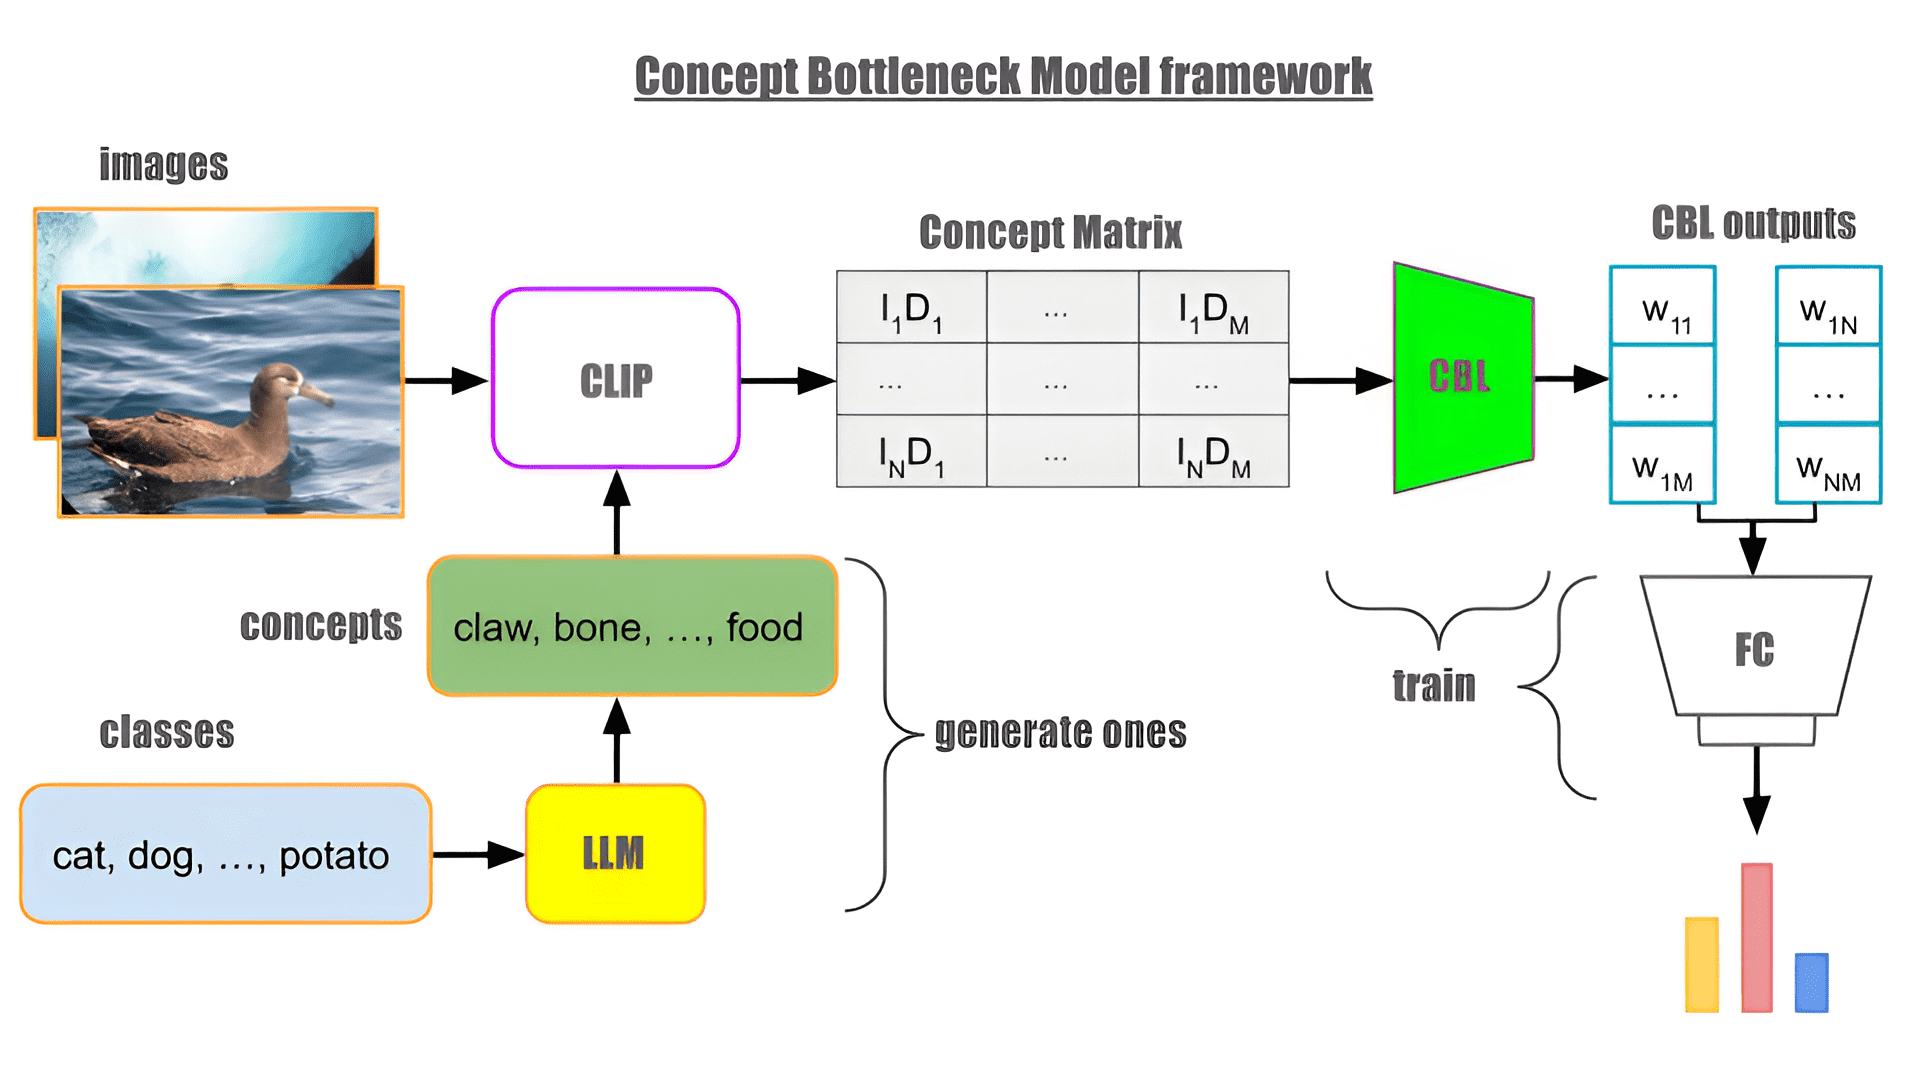
\includegraphics[width=1.\columnwidth]{./figures/framework-compressed.png}}
\caption{Архитектура фреймворка для построения CBM.}
\label{fig:framework}
\end{center}
\end{figure*}

В этом разделе мы предлагаем структуру, которая создает
Concept Bottleneck Model из предварительно обученного мультимодального кодера эффективным способом с минимальным количеством настраиваемых слоев и автоматической генерацией концептов для каждого рассматриваемого набора данных с точной настройкой. Сначала наш МД строит модель, подходящую для классификации изображений, а в качестве основы мы используем бимодальный кодер или CLIP-подобные модели, способные выдавать вкрапления или готовые к использованию оценки точечного произведения этих вкраплений. Это означает, что последний слой сети модифицируется в зависимости от количества классов в наборе данных. Во-вторых, количество концептов и их значение зависят только от меток набора данных и не меняются в процессе дальнейшего обучения. Мы можем кратко описать строительные блоки нашего фреймворка в виде следующих шагов:
\begin{itemize}
\item \textbf{Шаг 1:} Выберите подходящую мультимодальную модель, основанную на кодировании, в качестве основы (мы в основном используем OpenAI CLIP-ViT-L/14\footnote{В экспериментах мы используем модель Hugging Face \cite{wolf2020huggingfaces}, представленную на сайте \texttt{https://huggingface.co/openai/clip-vit-large-patch14}.}). Затем добавляем к ней два линейных слоя, первый из которых мы называем Concept Bottleneck Layer (CBL), как в \cite{oikarinen2023labelfree}, а второй - последний FC-слой.
\item \textbf{Шаг 2:} Выбираем набор данных, создаем набор концептов на основе меток классов и фильтруем\footnote{В экспериментах мы используем 'all-mpnet-base-v2' трансформатор предложений \cite{reimers-2019-sentence-bert} \nocite{reimers-2020-multilingual-sentence-bert}, присутствующий в \texttt{https://huggingface.co/sentence-transformers/all-mpnet-base-v2}.} нежелательных концептах.  
\item \textbf{Шаг 3:} Выбираем одну из наших целевых функций, упомянутых в разделах \ref{sec:sparsecbm}, \ref{sec:ellcbm}, \ref{sec:contrcbm} и два подходящих оптимизатора для полученной архитектуры (мы используем Adam \cite{kingma2017adam} и AdamW \cite{loshchilov2019decoupled}).
\item \textbf{Шаг 4:} Выучите CBL с подобранной на предыдущем шаге целью и FC с кросс-энтропийным лоссом.
\end{itemize}
Более конкретно. На \textbf{шаге 1} мы рассматриваем CLIP-подобную модель и добавляем к ней два линейных слоя. Для заданной партии входных изображений с \textbf{всеми} созданными концептами эта модель выводит оценки точечного произведения между конкретным изображением и всеми концептами, то есть, в терминах алгоритма CMS (раздел \ref{sec:cms}), мы получаем партию размером $|\mathrm{B}|$ строк матрицы $\mathcal{V}$. Эти оценки показывают, насколько чувствительны изображения от 1 до $|\mathrm{B}|$ к каждой концепции, поскольку более подходящие концепции получают более высокую оценку от CLIP. Первый линейный слой, назовем его CBL, управляет информативностью концептов, а второй FC делает окончательное предсказание. Мы храним CBL и FC как матрицы формы $|\mathrm{D}|\times|\mathrm{D}|$ и $|\mathrm{D}|\times|\mathrm{C}|$ соответственно. Единственное концептуальное различие между этими слоями заключается в том, как они обучаются. На \textbf{шаге 2} мы генерируем набор концептов. Как и в \cite{oikarinen2023labelfree}, мы не полагаемся ни на каких экспертов и создаем понятия вручную. Один из распространенных способов - создавать их, запрашивая у LLM метки классов и обрабатывая результаты работы LLM. Мы спрашиваем GPT-3 \cite{brown2020language}, Llama-2\footnote{В экспериментах мы используем бесплатную версию Llama-2, доступную на Hugging Face hub \texttt{https://huggingface.co/TheBloke/Llama-2-70B-Chat-GPTQ}. \cite{touvron2023llama} для этих целей}. Обе модели демонстрируют хорошее знание того, какие концепции более предпочтительны для каждого класса. Мы напрямую задаем следующий вопрос:

Prompt 1: "List the most important features for recognizing something as a \{label\}. Write them one by one."

Prompt 2: "List the things most commonly seen around a \{label\}. Write them one by one."

Prompt 3: "Give a generalization for the word \{label\}. Answer with a single sentence."

Также, в связи с правилами оплаты OpenAI API и размером моделей Llama-2, мы используем ConceptNet API \cite{article} для создания концептов также в автоматическом режиме, но более просто и бесплатно, как в \cite{oikarinen2023labelfree,yuksekgonul2023posthoc}. При использовании ConceptNet у нас нет возможности подсказывать, вместо этого мы используем Sentence Transformer \cite{reimers-2019-sentence-bert} и выбираем дальнейшие понятия с помощью алгоритма работы, аналогичного \cite{oikarinen2023labelfree}:

1) Чтобы представить понятия в виде нескольких слов, мы удаляем все понятия, длина которых превышает 30 букв.

2) Мы удаляем все понятия, у которых косинусоидальное сходство с классами больше 0,85.

3) Мы удаляем все понятия, у которых косинусоидальное сходство с другими понятиями больше 0,9 отсечки\footnote{0,85 для сходства "понятия-классы" и 0,9 для сходства "понятия-концепты" - это наши гиперпараметры, полученные эмпирическим путем, мы не собираемся менять их в дальнейших экспериментах}.

4) Мы удаляем понятия с меньшим средним сходством с другими понятиями, чтобы оставить более общие понятия. 

На \textbf{Шаг 4} мы, в свою очередь, предлагаем применить \textit{последовательное узкое место} схемы: пусть мы обучаем эти слои одновременно, но применяем оптимизатор FC ко всем обучаемым параметрам сети, кроме CBL, который обучается только со своим собственным оптимизатором. Если CLIP выдает $\psi(x, t) = \left(\langle i, d_1\rangle,\dots,\langle i, d_{|\mathrm{D}|}\rangle \right)^{\mathrm{\top}} \ в \mathbb{R}^{|\mathrm{D}|}$ с вложением изображения $i$ и вложением понятия $d_{\mathrm{j}}$ из набора данных $\mathcal{D} = (x, t, l)$, где $x$ обозначает визуальную модальность, $t$ обозначает \textbf{all} слова понятия, а $l$ - текстовое описание имени класса; функция потерь для CBL $\mathcal{L}_{\mathrm{CBL}}$; сама CBL $W_{\mathrm{CBL}}\in\mathbb{R}^{|\mathrm{D}|\times|\mathrm{D}|}$; и потери кросс-энтропии финального слоя и веса $\mathcal{L}_{\mathrm{CE}}$, $W_{\mathrm{F}}\in\mathbb{R}^{|\mathrm{C}|\times |\mathrm{D}|}$. Мы можем сформулировать период обучения для CBL следующим образом:
\[
\min \limits_{W_{\mathrm{CBL}}}\mathop{\mathbb{E}}_{(x, t, l)\sim\mathcal{D}}\big[\mathcal{L}_{\mathrm{CBL}}(W_{\mathrm{CBL}}\psi(x, t))\big]_,
\] и, на предыдущем шаге бэкварда, мы учим FC слой с
\[
\min \limits_{W_{\mathrm{F}}} \mathop{\mathbb{E}}\limits_{(x, t, l)\sim\mathcal{D}}\big[\mathcal{L}_{\mathrm{CE}}(W_{\mathrm{F}}W_{\mathrm{CBL}}\psi(x, t), l) \big]_.
\]
Таким образом, мы обучаем CBL и FC одновременно, но обновления градиента от Cross-Entropy loss не влияют на $W_{\mathrm{CBL}}$, что очень удобно при обучении слоев узких мест с $\ell_1$ или функций потерь Gumbel-Softmax, чтобы сделать эти слои разреженными. %%%%%%%%
Здесь мы показываем, что $\mathcal{L}_{\mathrm{CE}}$ ожидает двух аргументов в качестве типичной супервизорной потери, в то время как $\mathcal{L}_{\mathrm{CBL}}$ требует только одного аргумента в качестве самоподдерживающейся функции потерь. Для обоих уравнений мы используем оптимизаторы Adam или AdamW, подключенные к соответствующим слоям. Ключевое преимущество нашего фреймворка заключается в том, как обучить эту МД с двумя оптимизаторами: по одному для каждой из представленных выше задач; и какие функции потерь выбрать (см. разделы \ref{sec:contrcbm}, \ref{sec:sparsecbm}). А для случая обучения с потерями $\ell_1$ мы рассматриваем термин регуляризации, введенный в разделе \ref{sec:ellcbm}.

В \cref{fig:framework} мы приводим схему нашего общего фреймворка в виде архитектуры с настроенными слоями и генерацией концепций.

\subsection{Contrastive-CBM}
\label{sec:contrcbm}

В этом разделе мы предлагаем простую адаптацию потери CLIP для обучения концептуальных слоев. Использование контрастирующей цели вместо попытки предсказать точные слова, связанные с изображениями, - это то, что делает модель на основе CLIP популярной для классификации изображений с нулевого снимка и сходства изображений и текстов. Когда мы создаем МД на основе предварительно обученного мультимодального кодера и снабжаем его необходимым набором концептов, мы также можем свободно обучать его узкие слои с теми же контрастными потерями \cite{zhai2023sigmoid}. 

Но в нашем случае мы заставляем CBL обучаться, минимизируя не сходство CLIP "изображение-текст", а выходы слоя узкого места $W_{\mathrm{CBL}}\psi(x, t)$ с учетом параметров $W_{\mathrm{CBL}}$. Пусть $|\mathrm{B}|$ - размер партии, в которой задана мини-пария вкраплений $\mathrm{B} = \left((i_1, d_1, c_1), \dots, (i_{\mathrm{|B|}}, d_{\mathrm{|B|}}, c_{\mathrm{|B|}})\right)$. Для простоты мы приводим формулу для случая, когда количество концептов равно размеру партии $|\mathrm{D}| = |\mathrm{B}|$. Мы также обозначим $\varphi_{\mathrm{k}} \triangleq \left(\langle i_{\mathrm{k}}, d_{\mathrm{1}}\rangle, \dots, \langle i_{\mathrm{k}}, d_{|\mathrm{B}|}\rangle \right)^\top$ как вектор оценок точечного произведения между \textbf{all} концептами ($|\mathrm{D}| = |\mathrm{B}|$) и $k$-ым изображением из партии $\mathrm{B}$. В качестве $w_{\mathrm{k}}$ мы определяем $k$-ю строку матрицы $W_\mathrm{CBL}$. Тогда наши контрастные потери для обучения узкого слоя можно переписать следующим образом:
\begin{align*}\label{eq:contr}
-\frac{1}{2|\mathrm{B}|} \sum_{\mathrm{k}=1}^{|\mathrm{B}|}\Bigg(\log \frac{e^{\alpha \langle w_{\mathrm{k}}, \varphi_{\mathrm{k}}\rangle}}{\sum_{\mathrm{j}=1}^{|\mathrm{B}|}e^{\alpha \langle w_{\mathrm{k}}, \varphi_{\mathrm{j}}\rangle}} + \log \frac{e^{\alpha \langle w_{\mathrm{k}}, \varphi_{\mathrm{k}}\rangle}}{\sum_{\mathrm{j}=1}^{|\mathrm{B}|}e^{\alpha \langle w_{\mathrm{j}}, \varphi_{\mathrm{k}}\rangle}} \Bigg)_.
\end{align*}
Скаляр $\alpha$ параметризуется как $\exp{\tilde{\alpha}}$\footnote{В OpenAI CLIP $\tilde{\alpha} = 1.155$, который мы используем для CMS backbone CLIP, в то время как для CBM используется значение $2.659$}. Мы определяем "Contrastive-CBM" как частный случай концептуальной модели узких мест нашего фреймворка с контрастной целью $\mathcal{L}_{\mathrm{CBL}}$ для слоев узких мест в представленной выше форме. Мы также отмечаем, что этот вид потерь может быть эффективно реализован для распределенного обучения \cite{chen2023discoclip,zhai2023sigmoid}.

\subsection{Sparse-CBM}
\label{sec:sparsecbm}

В этом разделе мы предлагаем основную целевую функцию для обучения наших моделей. Во-первых, мы определяем распределение Gumbel-Softmax \cite{jang2017categorical,DBLP:journals/corr/MaddisonMT16} следующим образом: пусть $z$ - категориальная переменная с вероятностями $\pi_1,\cdots,\pi_{|\mathrm{D}|}$, то есть, $|\mathrm{D}|$-мерный однохотовый вектор из вероятностного симплекса $\Delta^{|\mathrm{D}|-1} \triangleq \{ \pi \in \mathbb{R}_+^{|\mathrm{D}|} : \sum_{i=1}^{|\mathrm{D}|} \pi_i =1 \}$. Тогда трюк Gumbel-max \cite{Gumbel1954StatisticalTO,maddison2015a} позволяет нам сделать выборку $z$ из категориального распределения с вероятностями классов $\pi = (\pi_1, \cdots, \pi_{|\mathrm{D}|})$:
\vskip -0.15in
\[
z = \mathbf{1}\left(\arg\max \limits_{\mathrm{k}}\big[g_{\mathrm{k}} + \log \pi_{\mathrm{k}}\big] \right)_,
\]
где $g_1,\dots, g_{|\mathrm{D}|}$ - i.i.d. выборки из $\mathrm{Gumbel}(0,1)$, которые, в свою очередь, могут быть получены из $u \ in \mathrm{Uniform}(0,1)$ путем выборки $g = -\log \log u$, (обозначим индикатор $\mathbf{1}$ как функцию одной точки). После применения функции softmax как непрерывной дифференцируемой аппроксимации к $\arg \max$ мы получаем распределение Гумбеля-Softmax, непрерывное распределение на симплексе, которое может аппроксимировать выборки из категориального распределения. Затем мы намерены построить контрастные потери для CBL-выводов следующим образом: 
\begin{align*}\label{eq:gumbellos}
-\frac{1}{2|\mathrm{B}|} \sum_{\mathrm{k}=1}^{|\mathrm{B}|}\Bigg(&\log \frac{e^{\left(\log(\alpha \langle w_{\mathrm{k}}, \varphi_{\mathrm{k}}\rangle) + g_{\mathrm{k}}\right)/\tau}}{\sum_{\mathrm{j}=1}^{|\mathrm{B}|}e^{\left(\log(\alpha \langle w_{\mathrm{k}}, \varphi_{\mathrm{j}}\rangle) + g_{\mathrm{j}}\right)/\tau}} \notag \\ 
&+ \log \frac{e^{\left(\log(\alpha \langle w_{\mathrm{k}}, \varphi_{\mathrm{k}}\rangle) + g_{\mathrm{k}}\right)/\tau}}{\sum_{\mathrm{j}=1}^{|\mathrm{B}|}e^{\left(\log(\alpha \langle w_{\mathrm{j}}, \varphi_{\mathrm{k}}\rangle) + g_{\mathrm{j}}\right)/\tau}} \Bigg)_.
\end{align*}

Мы используем полученную потерю для представления логитов слоя "узкого места" как категориальных переменных, т.е. разреженных векторов, которые хорошо интерпретируются \cite{pmlr-v139-wong21b}. С помощью структуры Гумбеля-Софтмакса $\mathcal{L}_{\mathrm{CBL}}$ достигается разреженное обучение слоев узкого места, что повышает их интерпретируемость: ключевым ингредиентом для обеспечения разреженности выходных векторов CBL является температура $\tau$. Представленное распределение является гладким для $\tau > 0$, оно имеет определенные градиенты по параметрам $w_{\mathrm{k}}$. Заменив категориальные выборки на выборки Гумбеля-Софтмакса, мы можем осуществлять обратное распространение через слои Concept Bottleneck. Для низких температур ($\tau < 0,5$) ожидаемое значение распределения Гумбеля-Софтмакса приближается к ожидаемому значению категориальной случайной величины с теми же логитами, т.е. становится одномоментным. С ростом температуры ожидаемое значение сходится к равномерному распределению по категориям. На практике мы начинаем с высокой температуры и отжигаем до небольшой, но ненулевой температуры.

\begin{figure}[h]
\begin{center}
\centerline{
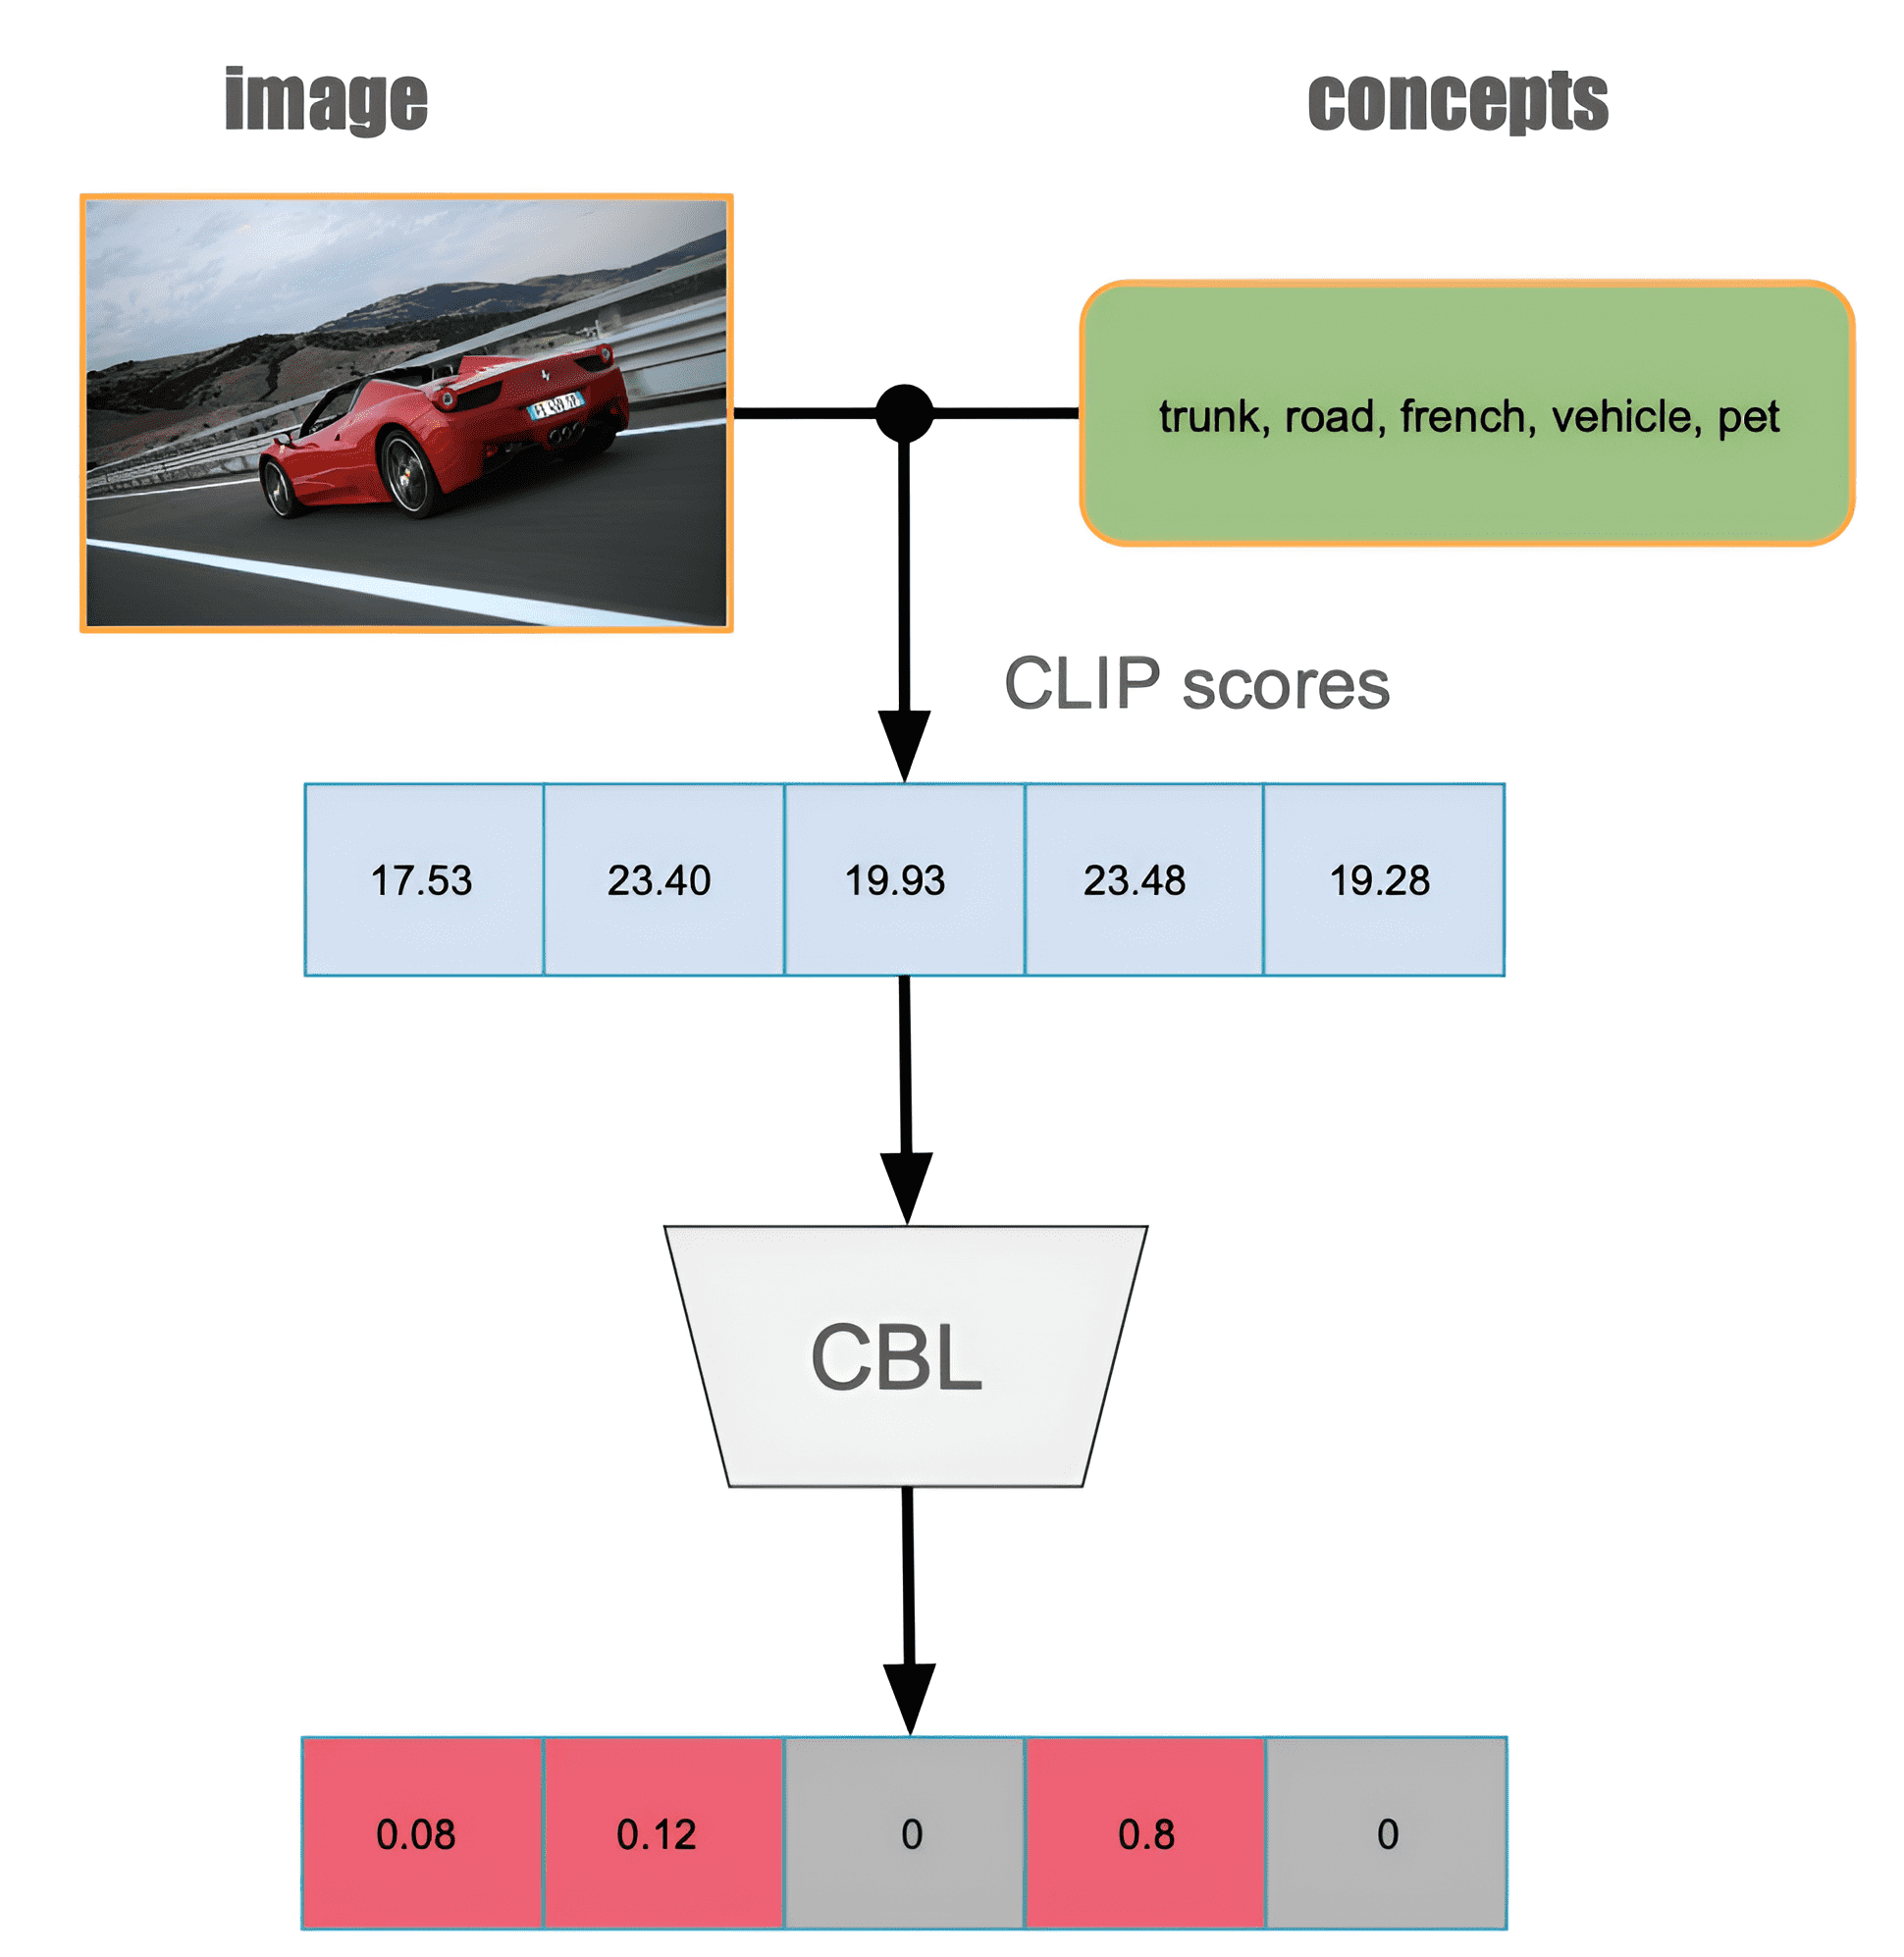
\includegraphics[width=0.6\columnwidth]{./figures/gumbel_example-compressed.png}}
\caption{Визуализация Sparse-CBM Concept Bottleneck слоев.}
\label{fig:gumbel_example}
\end{center}
\end{figure}
Если $\tau$ является обучаемым параметром (а не отжигается по фиксированному расписанию), эту схему можно интерпретировать как энтропийную регуляризацию \cite{szegedy2015rethinking,pereyra2017regularizing}. Высокоуровневое объяснение и вывод активаций Гумбеля можно посмотреть на \cite{alexandridis2022longtailed}.

\subsection{$\boldsymbol\ell_1$-CBM}
\label{sec:ellcbm}

Мы также обучаем концепт Bottleneck с помощью $\ell_1$-функции потерь. Ранее \cite{yuksekgonul2023posthoc} предлагал использовать штраф эластичной сети, а \cite{oikarinen2023labelfree} - среднее взвешенное между нормой Фробениуса и нормой матрицы элементов. Вместо этого мы показываем многообещающий результат только при использовании штрафа $\ell_1$. Штраф $\ell_1$ демонстрирует способность к спарсированию обучаемых слоев: оптимизатор пытается минимизировать потери, уменьшая веса, которые имеют ненулевой градиент, что приводит к тому, что некоторые веса устанавливаются точно в ноль, что эффективно удаляет соответствующие признаки из выходных данных CBL.

Начнем с определения следующей оптимизационной задачи:
\[
\min \limits_{W_{\mathrm{CBL}}} \mathop{\mathbb{E}}\limits_{(x, t, l)\sim\mathcal{D}}\big[\mathcal{L}_{\mathrm{CE}}(W_{\mathrm{F}}W_{\mathrm{CBL}}\psi(x, t), l) + \frac{\lambda}{|\mathrm{D}|}\Omega(W_{\mathrm{CBL}}) \big]_,
\]\label{eq:l1probl}где $\Omega(W_{\mathrm{CBL}})$ соответсвует регуляризатору. Мы используем:
\[
\Omega(W_{\mathrm{CBL}}) = \|W_{\mathrm{CBL}}\|_1
\] 
с единтвенной параметризацией $\lambda$. 